\chapter{Interrogazione dell'ontologia}

\section{SWRL}
Per permettere al reasoner di inferire maggiori informazioni riguardanti l'ontologia sono state realizzate alcune regole SWRL.

Le seguenti regole sono state realizzate per permettere al reasoner di inferire il valore di energia che una batteria può effettivamente assorbire o immettere.

Siccome varie sono le casistiche da controllare, sono state create quattro regole per i calcoli inerenti.

Per leggibilità sono stati inseriti gli screenshot delle regole, la versione testuale è disponibile nel file \href{https://github.com/19eddie/SemanticWeb-Assignment02-03/blob/main/SWRL%20energia%20che%20pu%C3%B2%20realmente%20assorbire%20o%20fornire%20una%20batteria.txt}{\textit{SWRL energia che può realmente assorbire o fornire una batteria.txt}
} reperibile su \href{https://github.com/19eddie/SemanticWeb-Assignment02-03}{Github}. \\

[\ref*{fig:bothlessorequal}] \texttt{Potenza massima di carica <= Capacità di carica e
    Potenza massima di scarica <= Capacità di scarica}

In questo caso la batteria può assorbire la \textit{potenza massima di carica} e può fornire la \textit{potenza massima di scarica}, ovvero .

\begin{figure}[H]
    \centering
    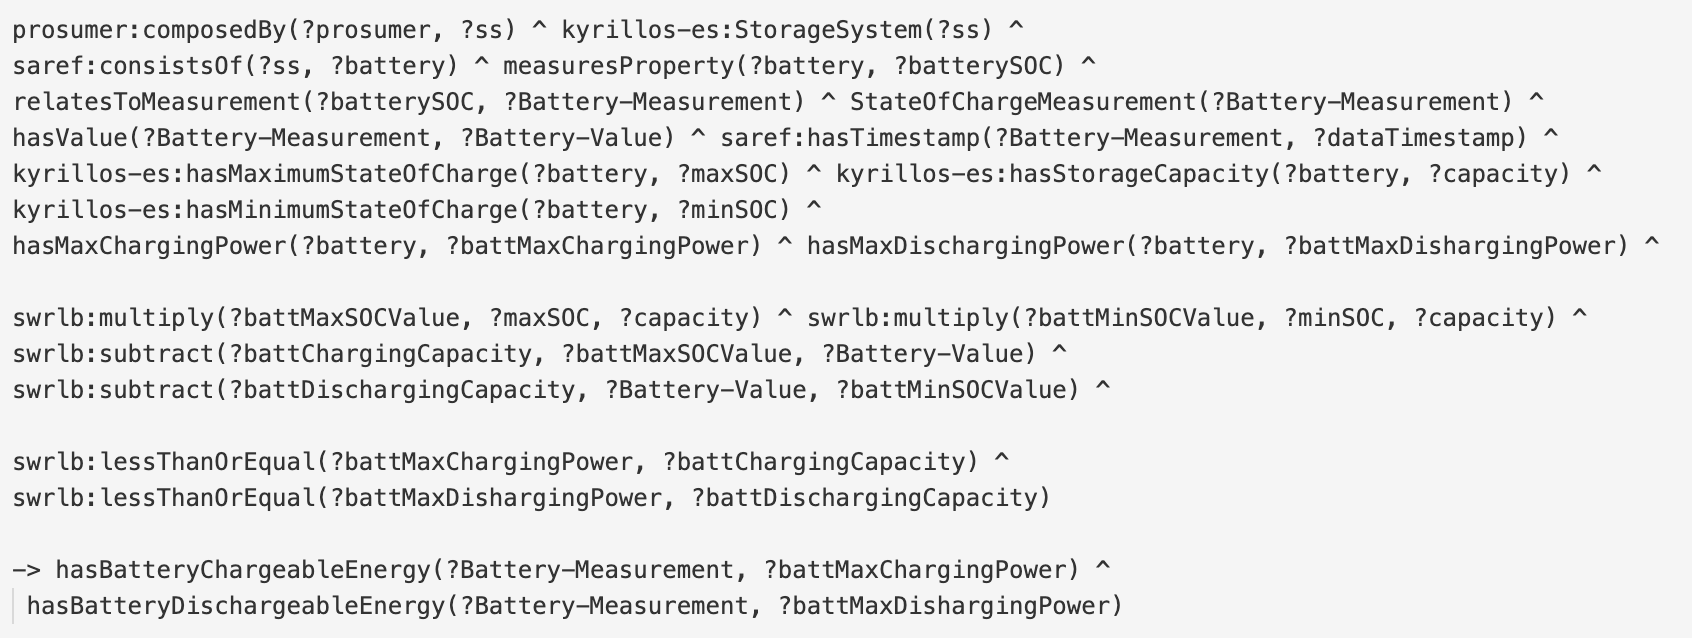
\includegraphics[width=15cm]{images/both <=.png}
    \caption{Screenshot della prima regola.}
    \label{fig:bothlessorequal}
\end{figure}

[\ref*{fig:charginglessorequal}] \texttt{Potenza massima di carica <= Capacità di carica e\\ Potenza massima di scarica > Capacità di scarica}

\begin{figure}[H]
    \centering
    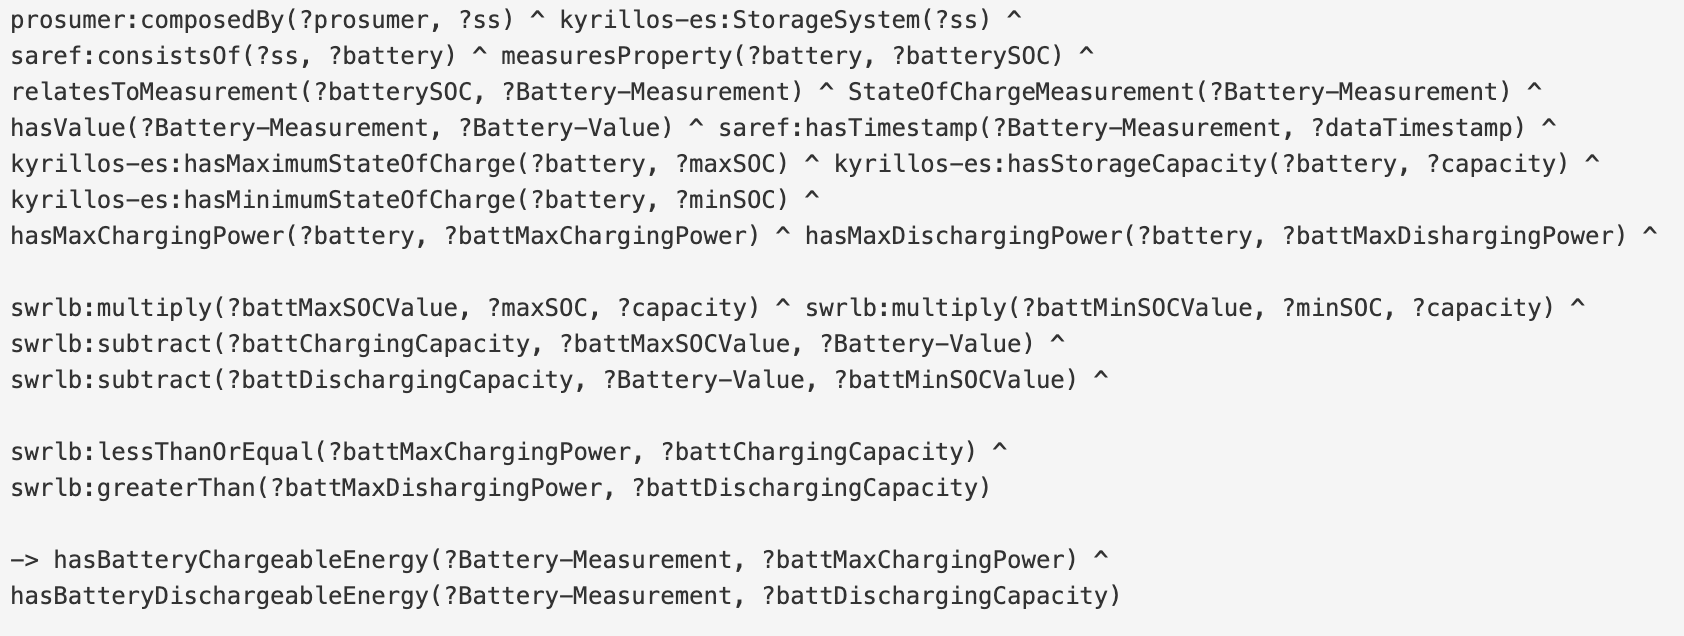
\includegraphics[width=15cm]{images/charging <=.png}
    \caption{Screenshot della seconda regola.}
    \label{fig:charginglessorequal}
\end{figure}

[\ref*{fig:charginggreater}] \texttt{Potenza massima di carica > Capacità di carica e\\ Potenza massima di scarica <= Capacità di scarica}

\begin{figure}[H]
    \centering
    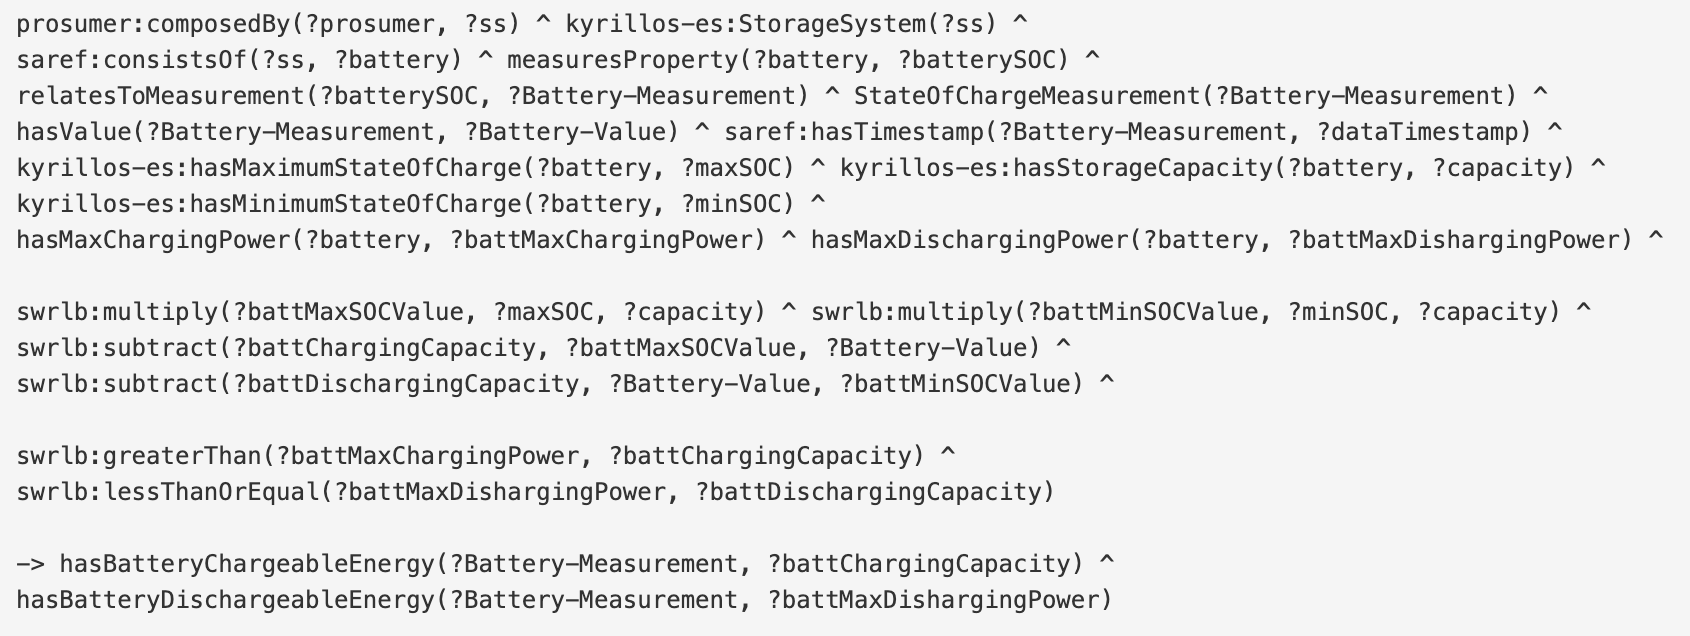
\includegraphics[width=15cm]{images/charging >.png}
    \caption{Screenshot della terza regola.}
    \label{fig:charginggreater}
\end{figure}

[\ref*{fig:bothgreater}] \texttt{Potenza massima di carica > Capacità di carica e\\ Potenza massima di scarica > Capacità di scarica}

\begin{figure}[H]
    \centering
    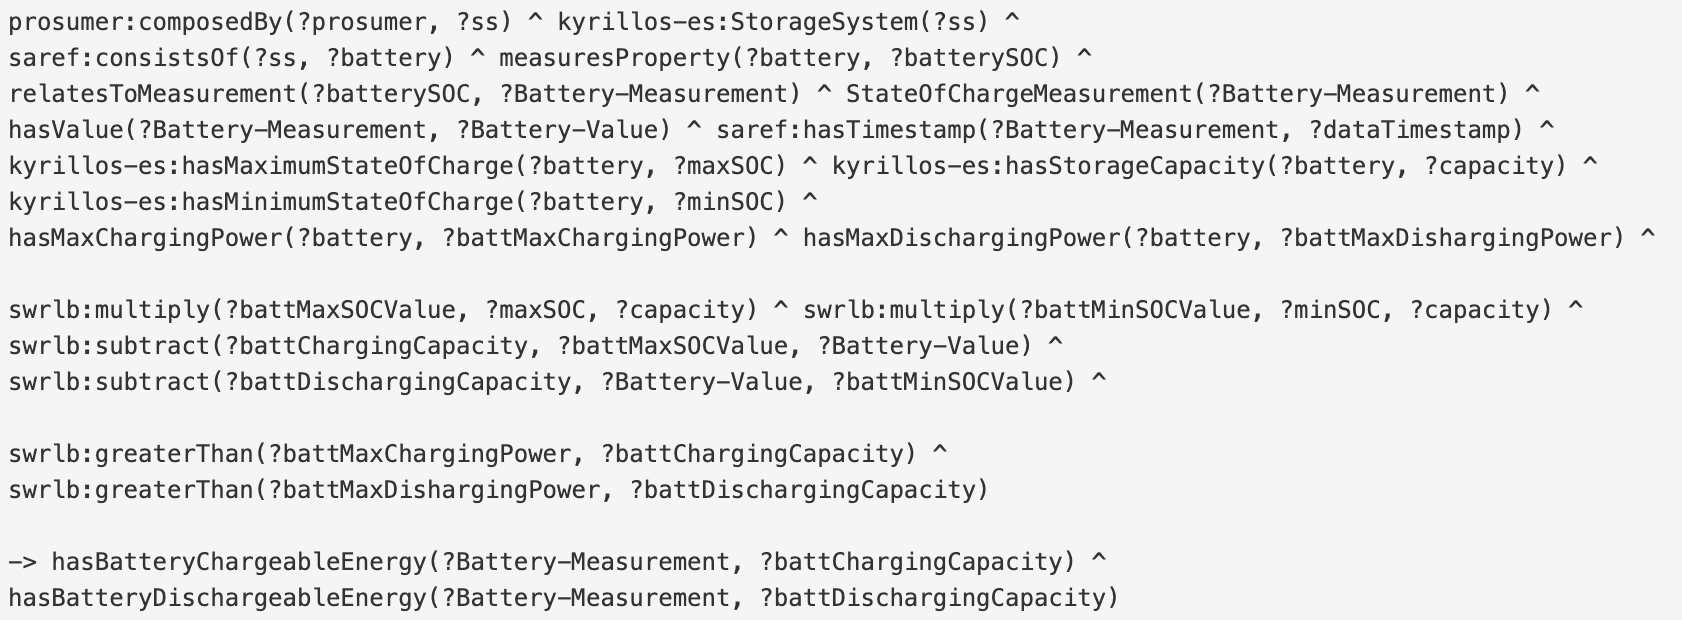
\includegraphics[width=15cm]{images/both >.png}
    \caption{Screenshot della quarta regola.}
    \label{fig:bothgreater}
\end{figure}

\section{SPARQL}
Nella seguente sezione verranno mostrate le query SPARQL e relativi risultati applicati agli individui creati nell'ontologia.

Si nota che per praticità, siccome sono query molto lunghe, verranno mostrate solamente parti delle query e i risultati, mentre le query complete sono disponibili nei relativi file di testo che verranno linkati.

\subsection{PREFIX}
Per leggibilità i prefissi utilizzati per le query SPARQL verranno visionati solamente in questa sezione.

\begin{figure}[H]
    \centering
    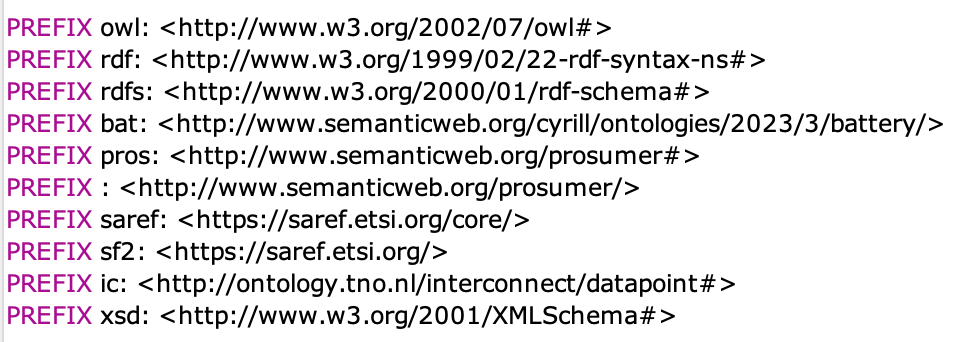
\includegraphics[width=15cm]{images/prefissi.png}
    \caption{Prefissi da anteporre alle query sull'ontologia.}
    \label{fig:prefix}
\end{figure}

\subsection{Query che calcola l'energia che può fornire o assorbire uno Storage System}

\begin{figure}[H]
    \centering
    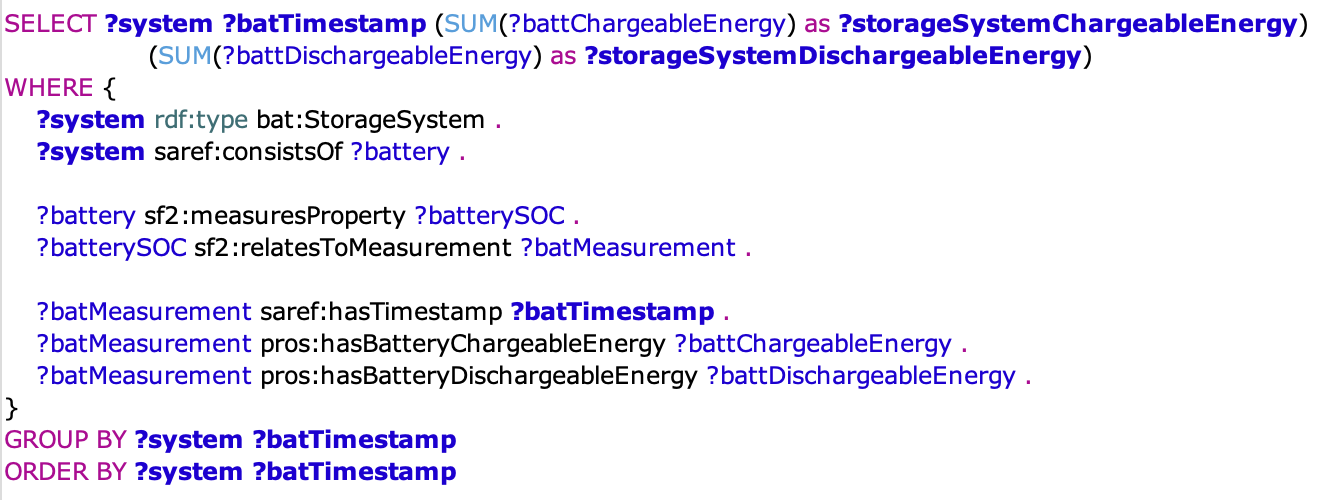
\includegraphics[width=15cm]{images/subquery.png}
    \caption{Query per il calcolo dell'energia che uno Storage System può assorbire o fornire.}
    \label{fig:subquery}
\end{figure}

\begin{figure}[H]
    \centering
    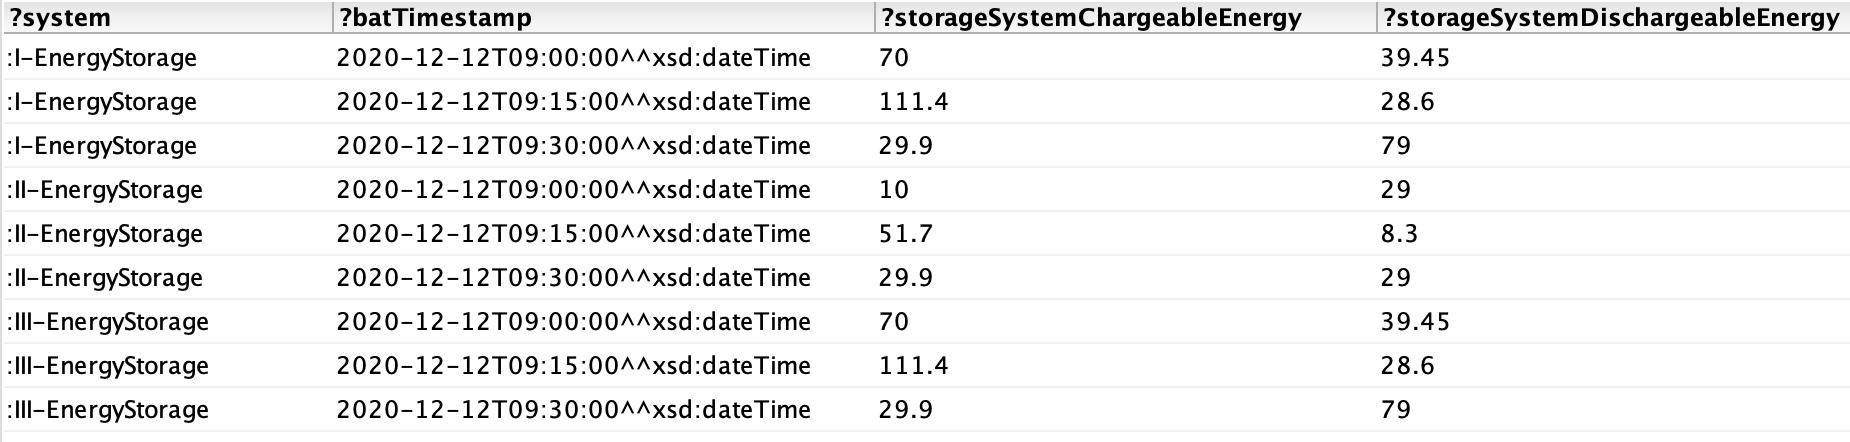
\includegraphics[width=15cm]{images/subquery_res.png}
    \caption{Risultati della query per il calcolo dell'energia che uno Storage System può assorbire o fornire.}
    \label{fig:subquery_res}
\end{figure}

\subsection{Query sul calcolo della flessibilità del contatore M1}

\subsection{Query per il calcolo di M1 e M2 in prosumer di configurazione 1 e 2}

\subsection{Query per il calcolo di M1, M2 e M3 in prosumer di configurazione 3}